\chapter{Introduction}
\label{ch:internship-intro}

\section{Company}

During the final semester of my studies at the Athens University of Economics
and Business, Greece, from March to June 2024, I completed my internship at
Ernst \& Young Greece, with my internship supervisor being Mr. George Kolomvos,
Senior Manager at Data \& AI Department of Ernst \& Young Greece. My internship
choice was based on my interest in data analytics and artificial intelligence,
and my desire to gain practical experience in the field. I particularly chose
Ernst \& Young Greece due to its reputation as a leading professional services
provider and also because I had the opportunity to visit the company's offices
and meet with some of the professionals working there during a company
presentation that the University organized. This experience gave me a positive
impression of the company's culture, values, and the work environment, and I
was eager to learn more about the services it offers and the projects it
undertakes.

% Info about the company
Ernst \& Young is a multinational professional services firm headquartered in
London, England. EY is one of the largest professional services firms in the
world and is one of the "Big Four" accounting firms. EY operates as a network
of member firms which are separate legal entities in individual countries. It
has 284,000 employees in over 700 offices around 200 countries in the world. It
provides assurance (including financial audit), tax, consulting and advisory
services to companies. The firm dates back to 1849 with the founding of Harding
\& Pullein in England. The current firm was formed by a merger of Ernst \&
Ernst (U.S.) and Arthur Young \& Co. (U.S.) in 1989. It was known as Ernst \&
Young until a rebranding campaign officially changed the name to EY in 2013
\cite{Ey}.

% More info about the company
EY is known for its commitment to building a better working world by helping
clients solve their toughest challenges, realize their ambitions, and create
sustainable value for their stakeholders. The firm's core values include
integrity, respect, teamwork, and professionalism. EY's services are designed
to help clients navigate the complexities of the business world, manage risks,
and seize opportunities for growth and innovation. The firm's global reach and
diverse expertise enable it to deliver high-quality services to clients across
a wide range of industries and sectors.

EY operates with a global structure that is divided into four main service
lines:

\begin{itemize}
    \item \textbf{Assurance:} This service line includes financial audit and accounting services. It ensures the accuracy and reliability of financial information provided by clients.
    \item \textbf{Tax:} This service line offers a range of tax advisory services, including corporate tax, international tax, transaction tax, and indirect tax services.
    \item \textbf{Advisory/Consulting:} This includes performance improvement, risk management, technology consulting, and strategy services. The consulting division helps clients improve their business performance and manage risk.
    \item \textbf{Strategy and transactions:} This service line focuses on providing clients with advice on transactions, mergers, acquisitions, and corporate restructuring. It also includes advisory services on regulatory compliance and business strategy.
\end{itemize}

Each of these service lines is further divided into various industry sectors,
allowing EY to provide specialized knowledge and expertise to clients in
different markets. Below we can see the general organizational chart of Ernst
\& Young, and in more detail of the Consulting Department, where I was assigned
during my internship \ref{fig:ey-structure}.

\begin{figure}[H]
    \centering
    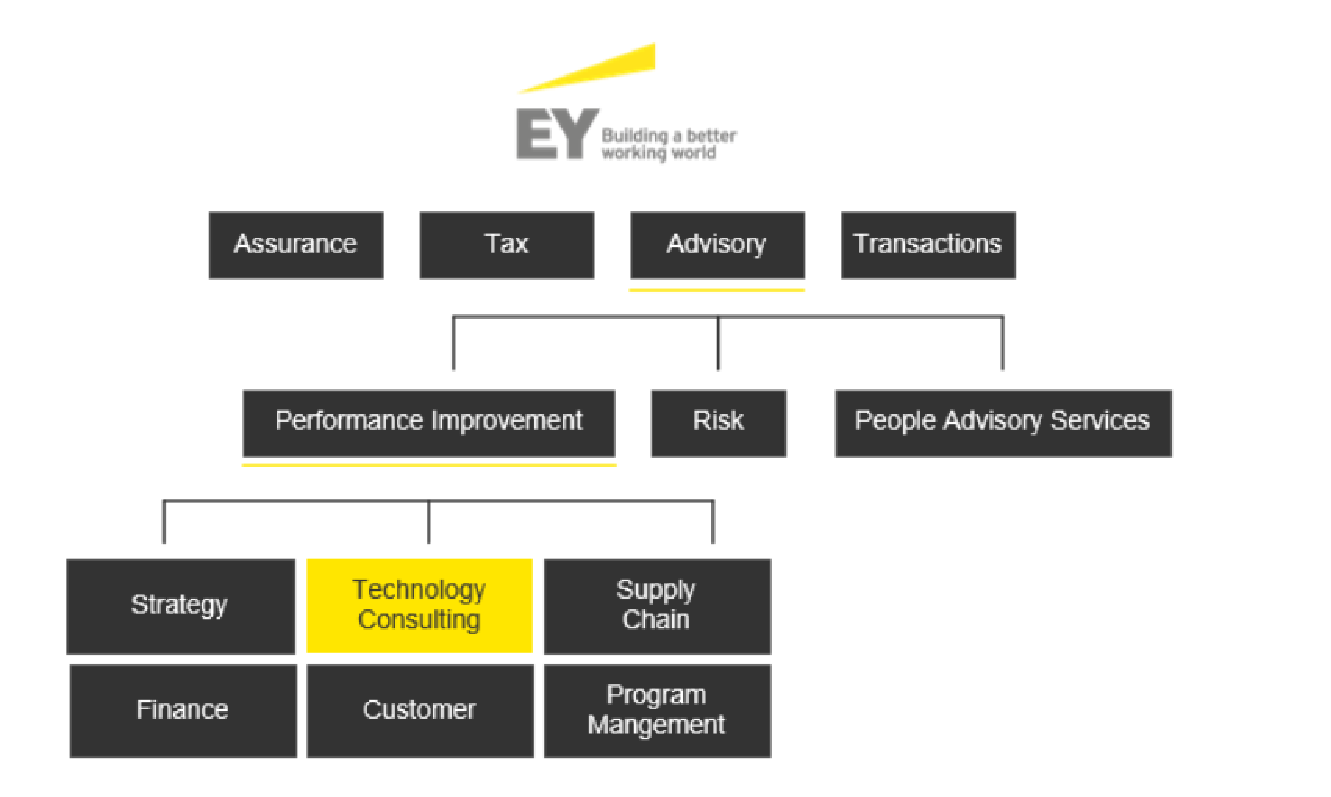
\includegraphics[width=\textwidth]{../figs/org_chart}
    \caption{Ernst \& Young Organizational Structure}
    \label{fig:ey-structure}
\end{figure}

\section{Internship Goals}

The main goal of my internship at Ernst \& Young Greece was to gain practical
experience in the field of data analytics and artificial intelligence. I aimed
to apply the knowledge and skills I acquired during my studies to real-world
scenarios, specifically by utilizing both my Major in Software Engineering and
Data Science and my Minor in Management of Information Systems and E-Business.
My specific objectives included:

\begin{itemize}
    \item \textbf{Application of Academic Knowledge:} To apply theoretical knowledge from my coursework in Software Engineering and Data Science to practical projects within the Data \& AI Department.
    \item \textbf{Industry Processes and Methodologies:} To learn about and engage with the processes and methodologies used in the industry, gaining insights into best practices for data analytics and artificial intelligence implementation.
    \item \textbf{Professional Skill Development:} To enhance my professional skills, including project management, teamwork, and communication, while working in a corporate environment.
    \item \textbf{Network Expansion:} To expand my professional network by connecting with industry experts, colleagues, and mentors within the Data \& AI field.
    \item \textbf{Business Operations Insight:} To gain a deeper understanding of the business operations of a large professional services firm, and how data analytics and artificial intelligence are leveraged to drive business value for clients.
    \item \textbf{Contribution to Projects:} To contribute to ongoing projects within the Data \& AI Department, delivering high-quality work that adds value to the team and clients.
    \item \textbf{Familiarity with Tools and Technologies:} To become proficient with industry-standard tools and technologies, such as advanced data analytic techniques and software, by working on real-world projects.
\end{itemize}

Ultimately, my internship aimed to bridge the gap between academic knowledge
and industry practice, providing me with valuable experience and insights that
would prepare me for a successful career in data analytics and artificial
intelligence.

\section{Goal of the Report}

The main purpose of this report is to summarize the knowledge acquired during
the internship at EY as well as to provide an overview of the activities and
projects I was involved in. Through the implementation of my final report, I
attempt to evaluate the knowledge, experience, and overall impact of my
internship. This report provides a thorough description of my three-month
activities and evolution at EY, my final thoughts on the company, my colleagues
and supervisors, the project I worked on, and the benefits I earned.